\documentclass[12pt, a4paper]{scrartcl}
\usepackage{geometry}
\geometry{
	left=2.5cm,
	right=2cm,
	top=2.5cm,
	bottom=3cm,
	%bindingoffset=5mm
}

\usepackage [T1]{fontenc}
\usepackage [utf8]{inputenc}
\usepackage [ngerman]{babel}

\usepackage{times}

\usepackage{booktabs} %minipages
\usepackage{wrapfig} %Tabellen/ Grafiken mit umschließendem Text
\usepackage{upgreek} % Griechische Großbuchstaben
\usepackage{textcomp} % Nur für das Promille-Zeichen
\usepackage{graphicx} % Required for the inclusion of images

\usepackage{fancyhdr} % Angepasste Kopf-/ Fußzeilen
\pagestyle{fancy}
\renewcommand{\headrulewidth}{0pt}%0.4 Standard
\renewcommand{\footrulewidth}{0pt}%0.4 Standard
\fancyhead{} %leert den Head
\fancyfoot{} % leert den Foot
\fancyfoot[L]{\small{Lastenheft Sprachassistent-Raumverwaltung}} % alles, was im linken Teil steht. Falls die Schriftgröße geändert werden soll, dann \fontsize{<size>}{<baselineskip}\selectfont (Schriftgröße, dann Text mit festgelegtem Standardabstand zwischen den Worten - Baselineskip)
\fancyfoot[C]{\small{Gruppe 3.4}}
\fancyfoot[R]{\thepage} %Seitennummer

\newcommand\tab[1][1cm]{\hspace*{#1}}

%\usepackage[
%backend=bibtex,
%style=phys,]
%{biblatex}
%\addbibresource{quellen.bib}
%%\AtEveryCite{\color{blue}}

\usepackage{amsmath} % Required for some math elements
%\usepackage{lineno} % Zeilennummerierung
%\renewcommand\linenumberfont{\normalsize} %Macht die Zeilennummerierung normalgroß (anstatt \tiny)
%\usepackage{romannum} % Römische Nummern, \romannum {1} - klein, \Romannum {1} groß

\usepackage{url} %Für das Zitieren von URLs
\usepackage{caption}
\usepackage[
colorlinks=true,
urlcolor=blue,
linkcolor=black
]{hyperref} % Internet-Links im Text klickbar machen
\usepackage{xcolor}

\setlength\parindent{0pt} % Removes all indentation from paragraphs

%\modulolinenumbers[5] %Nummeriert nur jede 5. Zeile
\captionsetup{justification=raggedright,singlelinecheck=false}

\usepackage[numindex,numbib]{tocbibind} %Au­to­mat­i­cally adds the bib­li­og­ra­phy and/or the in­dex and/or the con­tents, etc., to the Ta­ble of Con­tents list­ing. 
%\renewcommand{\listoffigures}{\begingroup
%	\tocchapter
%	\tocfile{\listfigurename}{lof}
%	\endgroup}
%
%\renewcommand{\listoftables}{\begingroup
%	\tocsection
%	\tocfile{\listtablename}{lot}
%	\endgroup}

\begin{document}
	\title{Sprach- und Raumverwaltung mittels Sprachassistent an der W-HS Bocholt}
	\subtitle{Praktikumsaufgabe 5: Lastenheft\\
	\large Softwaretechnik I - WS 2017/ 2018}
 
	\author{Gruppe 3.4\\
		Lennart Bierwolf\\Daniel Großenbach\\Maximilian Krings}
	\maketitle
	\thispagestyle{fancy} %Fancy-Header wird auf diese Weise auch auf die Titelseite angewandt
	\begin{center}
		
	\end{center}

%\begin{center}
%\tab Gruppe 3.4
%\end{center}

\newpage
	
\tableofcontents
\newpage
\section{Zusammenfassung}
Zur Bewertung der verfügbaren Sprachassistenz-Technologien soll im Rahmen eines Semesterprojekts eine rechnergestützte, per Sprache steuerbare Stundenplan- und Raumverwaltung am Campus Bocholt der Westfälischen Hochschule entworfen werden. Die Verwaltung soll dabei sämtliche Informationen des schon vorhandenen Stunden- und Raumplans in Sprachform zurückgeben können und mit dem Websystem der bereits existierenden, regulären Raum- und Stundenplan-Verwaltung interagieren können. Weiterhin soll es möglich sein, Planänderungen per Sprache durchzuführen.\\
\\
Dieses Lastenheft charakterisiert die allgemeinen Anforderungen, die an die Sprachverwaltung gestellt werden. Neben den notwendigen Qualitätsanforderungen an die Software werden noch -soweit möglich- die zu erfüllenden Bedingungen angegeben, damit das System in einer unruhigen, lauten Umgebung mit zufriedenstellender Qualität funktionieren kann. Besonders wichtig ist, dass die Sprachverwaltung im normalen Betrieb nicht auf einen Bildschirm zurückgreifen können soll, sondern mit dem Nutzer ausschließlich per Ton kommuniziert. Deswegen muss die Bedienbarkeit auch möglichst simpel und schnell sein, damit auch unter Zeitdruck stehende Nutzer zuverlässig die gewünschten Informationen erhalten können. Da verschiedene Technologien zum Einsatz kommen sollen, muss außerdem das System stark modularisiert gebaut werden, damit ein möglichst problemloser Wechsel zwischen den Technologien ermöglicht werden kann.\\
\\
Darüber hinaus werden in dem Lastenheft die einzelnen Nutzergruppen (unregistrierter Benutzer, registrierter Benutzer,  Dozent und System-Administrator) und überblicksartig die für die jeweiligen Gruppen zur Verfügung stehenden Funktionalitäten beschrieben. Die Nutzergruppen beinhalten dabei die Eigenschaften und üblichen Tätigkeiten jeder Gruppe.

\section{Zielbestimmung}
Das ultimative Ziel dieses Projekts ist es, eine Sprachassistenz-Technologie derart mit dem vorhandenen Stunden- und Raumplanungssystem zu verknüpfen, dass detaillierte Abfragen von Planinformationen komfortabel per Sprachbefehl gestellt werden und mindestens genauso schnell wie beim bereits vorhandenen System erhalten werden können.\\
\\
Auf dem Weg zu diesem Ziel werden zusätzlich verschiedene Assistenz-Technologien bewertet: Dafür soll zunächst die im Vorhinein als am besten geeignete Technologie eingesetzt werden. Falls diese sogar noch besser als gedacht die Erwartungen erfüllt, müssen andere Technologien nicht mehr weiter erprobt werden. Ansonsten sollen aber mehrere Technologien getestet werden und, soweit möglich, jederzeit austauschbar sein.

\newpage

\section{Einsatz- und Benutzerprofile}

\subsection{Einsatz}
Die Sprachverwaltung soll als Client-/Serversystem realisiert werden. Der zentrale Server wird von der Westfälischen Hochschule, Abt. Bocholt (W-HS) zur Verfügung gestellt. Die Clients treten in zwei Formen auf: Zum einen können sie Konsolen sein, die - mit Mikrophon und Lautsprecher ausgestattet - an mehreren zentralen Punkten im  Gebäude der W-HS aufgestellt sind. Anfragen an diesen Konsolen können entweder mit einem Knopfdruck oder einer Audiopassphrase begonnen werden. Diese Form der Clients reicht die eingehenden Sprachanfragen und -befehle an den Server weiter und gibt die Antwort in Audioform wieder aus. Dozenten ist es auch nach einer vorherigen Registrierung möglich, die zugrundeliegenden an den Konsolen Pläne zu ändern.\\
Die andere Client-Form ist webbasiert: Ein Nutzer kann sich mit an einem Computer mit Netzwerk-Zugang im Browser anmelden und dort das zuvor registrierte Nutzerkonto konfigurieren. Sämtliche Anmeldungen benötigen eine gültige Nutzerkennung und ein zugehöriges Passwort. Weiterhin ist es analog zur Konfiguration via Sprache möglich, über eine Schnittstelle zur regulären Raum- und Stundenplanung Veränderungen an den Stunden- und Raumplänen vorzunehmen (entsprechende Berechtigungen vorausgesetzt).\\
Einem Benutzer können mehrere Profile zugeordnet werden (beispielsweise kann ein Dozent auch Administrator sein), für die er durch die Zuordnung authentifiziert wird. Einzig und allein nicht registrierte Benutzer sind davon ausgeschlossen.\\
\\
Es kann je nach verwendeter Sprachassistenz-Technologie nötig sein, eine Verbindung zum Internet zu haben. Allgemein soll 
aber bei vergleichbarer Qualität eine nicht internetbasierte Technologie bevorzugt werden.

\subsection{Benutzerprofile}
Für das System sind 4 allgemeine Benutzerprofile vorgesehen, die im folgenden Diagramm überblicksartig mit ihrer Hierarchie dargestellt werden:

\begin{figure}[h!]
		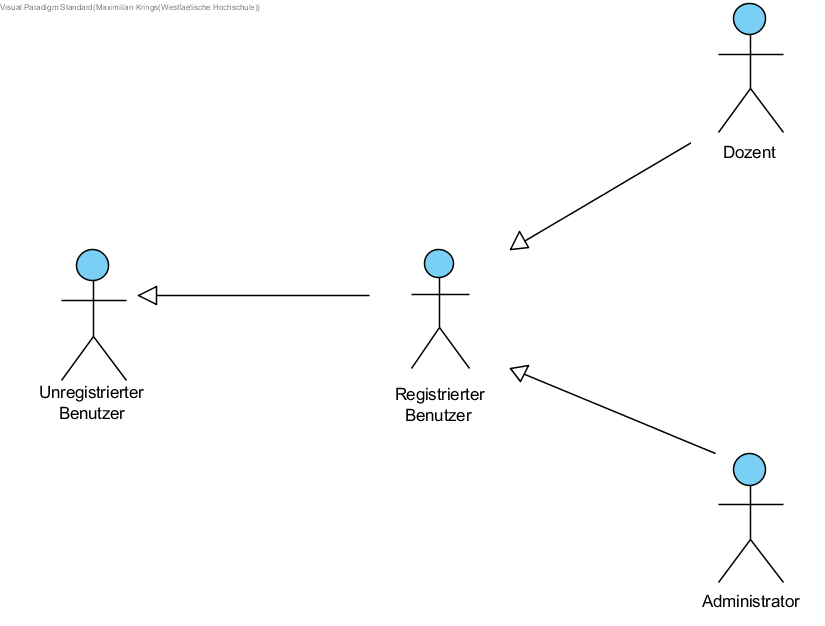
\includegraphics[width=0.6\textwidth]{nutzer.png}
	\caption{\emph{Hierarchie der Benutzerprofile}}
	\label{fig:hierarchie}
\end{figure}

\subsubsection{Registrierter Benutzer}
Registrierte Benutzer haben mit ihnen zur Verfügung stehenden Login-Daten  einen Account angelegt und können sich mit diesem auf dem webbasierten Client anmelden. Ein registrierter Benutzer kann auf der Webseite der Plattform eintragen, für welchen Studiengang er eingetragen ist, in welchem Semester er ist und welche Vorlesungen von ihm besucht werden (beziehungsweise für Dozenten, welche Vorlesungen er hält). Diese \emph{zusätzlichen Angaben} sind optional und sollen ermöglichen, eine bessere (schnellere) Antwort bei Anfragen über das Sprachportal zu ermöglichen.\\
Jedem registrierten Account wird eine eindeutige, von dem Accountnamen verschiedene User-ID zugeordnet, die zur Identifikation über das Sprachportal genutzt werden kann und darauf aufbauend mit den zusätzlichen Angaben eine schnellere Antwort ermöglicht (sofern die zusätzlichen Angaben eingetragen wurden). Ein registrierter Benutzer ohne weitere Berechtigungen (in Form von zusätzlich zugeordneten Benutzerprofilen) gilt automatisch als Studierender. Die Registrierung ist, sofern ein Nutzer nur die Rolle eines Studierenden einnimmt, optional und dient der höheren Präzision der Sprachantwort (das Nennen der zuvor eingetragenen zusätzlichen Angaben muss nicht mehr vorgenommen werden). Ansonsten hat ein registrierter Benutzer sämtliche Funktionen eines unregistrierten Benutzers.

\subsubsection{Unregistrierter Benutzer}
Ein unregistrierter Nutzer kann an der Sprachkonsole einen Studiengang und Semester nennen und gleichzeitig Anfragen stellen. Ein Nutzer gilt bei Anfragen als nicht registriert, wenn er zu Beginn seiner ersten Anfrage nicht seine ihm zugeordnete ID nennt. Unregistrierte Benutzer können nur über die Sprachkonsolen mit dem System interagieren.

\subsubsection{Dozent}
Ein Dozent bietet Lehrveranstaltungen und Prüfungen für Studierende an. Er kann für die ihm zugeordneten Veranstaltungen und Prüfungen den Raum und die Zeit ändern und ggf. weitere Teilveranstaltungen (beispielsweise ein zusätzliches Praktikum) anbieten.

\subsubsection{Administrator}
Der Administrator ist für die Wartung und Verwaltung der Sprachassistenten-Verwaltung zuständig. Er kann die Benutzerprofile der registrierten Benutzer verwalten und das System mithilfe von Backups sichern und aus diesen Backups einen Systemzustand wiederherstellen. Außerdem ist es ihm möglich, zwischen verschiedenen Sprachtechnologien zu wechseln.

\newpage

\section{Produktfunktionen}
In diesem Abschnitt werden die Funktionen, die das System jeder Benutzergruppe zur Verfügung stellt, grob aufgelistet und die Beziehungen der einzelnen Gruppen zueinander kurz genannt.

\subsection{Registrierter Benutzer}
Registrierte Benutzer haben alle Rechte und Funktionen von unregistrierten Benutzern und darüber hinaus folgende Funktionen:
\begin{itemize}
	\item An-/Abmeldung auf der Webplattform
	\item Zusätzliche, optionale Angaben über Studiengang, Semester, besuchte Veranstaltungen (für Studenten) / Lehrveranstaltungen (für Dozenten). Dienen nur der schnelleren Abfrage. Können jederzeit geändert werden.
	\item Zuordnung einer eindeutigen ID nach der Registrierung
	\item Änderung des eigenen Passworts
\end{itemize}
\subsection{Unregistrierter Benutzer}
 Die folgenden Anfragen können aneinandergereiht an das System gestellt und auf diese Weise kombiniert werden:
\begin{itemize}
	\item Alle verbleibenden Veranstaltungen am aktuellen Tag ausgeben
	\item Alle Veranstaltungen an einem beliebigen Tag ausgeben (auch Veranstaltungen, die an einem bestimmten Datum einmalig stattfinden)
	\item Raumnummer einer Veranstaltung
	\item Name [einer/ aller] Veranstaltung[en] ausgeben, die an einem bestimmten Wochentag zu einer bestimmten Uhrzeit stattfindet[stattfinden]
	\item Belegungsplan eines Raums ausgeben
	\item Belegungsstatus eines Raums eines bestimmten Typs/ mit einer bestimmten Ausstattung
	\item Falsche Anfragen können korrigiert werden
\end{itemize}

\subsection{Dozent}
Dozenten werden aus registrierten Benutzern abgeleitet (siehe Abbildung \ref{fig:hierarchie}). Dabei wird die Möglichkeit, bei den zusätzlichen Angaben Informationen über das Semester und den Studiengang zu machen, entfernt und stattdessen durch Angaben über seine Lehrveranstaltungen ersetzt.
\begin{itemize}
	\item Kann (kurzfristig) den Raum und den Beginn einer seiner (Teil-)Veranstaltungen ändern oder diese ausfallen lassen
	\item seine Veranstaltungen als zusätzliche Angaben eintragen
	\item mithilfe seiner ID seine Lehrveranstaltungen per Sprachkonsole ausgeben lassen
	\end{itemize}

\newpage

\section{Produktdaten}

Dieser Abschnitt umreißt die Eigenschaften von Lehrveranstaltungen und Räumen. Die Sprachtechnologie muss ein Verständnis dieser Eigenschaften besitzen und sie ggf. verändern können. Im Raum- und Stundenplan sind (Teil-)Lehrveranstaltungen und Räume fest miteinander verknüpft.

\subsection{Lehrveranstaltung}
Eine Lehrveranstaltung hat eine eindeutige ID, ein Kürzel und eine kurze Beschreibung. Ein oder mehrere Dozenten bieten die Lehrveranstaltung an und können sie modifizieren. Die Lehrveranstaltung kann (muss aber nicht) aus verschiedenen Teilveranstaltungen (Vorlesung, Übung, Praktikum) bestehen, wobei jede dieser Teilveranstaltungen in unterschiedlichen Räumen zu einer unterschiedlichen Zeit stattfinden kann. Es kann auch mehrere Teilveranstaltungen gleichen Typs geben. Eine Lehrveranstaltung ist einem Fachbereich fest zugeordnet, kann aber von Mitgliedern anderer Fachbereiche ebenfalls besucht werden.

\subsection{Raum}
Ein Raum hat eine eindeutige Nummer, eine Sitzplatzkapazität und ist von einem bestimmten Typ (z.B. Hörsaal, Seminarraum, Labor). Außerdem hat jeder Raum eine Ausstattung (Tafel, Computerplätze, Beamer, Overhead-Projektor, ..), die von Raum zu Raum unterschiedlich sein kann. Ein Raum gilt als belegt, wenn eine Veranstaltung zu einer bestimmten Zeit in diesem Raum stattfindet.

\section{Qualitätsanforderungen und Akzeptanzkriterien}

\subsection{Funktionalität und Effizienz}
Die beiden Client-Typen werden in diesem Abschnitt getrennt betrachtet.
\subsubsection{Sprachkonsolen}
Die Sprachkonsolen sind von Montag bis Freitag innerhalb der Öffnungszeiten der Fachhochschule (7:00 bis 21:30 Uhr) ständig verfügbar. Den Konsolen ist es allerdings gestattet, nach 15 Sekunden ohne Benutzereingabe in den Standby-Modus zu wechseln, in dem sie verbleiben dürfen, bis ihnen entweder durch Knopfdruck oder durch einen expliziten Sprachbefehl eine Aktivität signalisiert wird.\\
Da die Konsolen an belebten Punkten in der Fachhochschule aufgestellt werden, muss die Hardware (Mikrofon und Lautsprecher) in der Lage sein, auch bei erhöhten Lautstärken und mit störenden Hintergrundgeräuschen sowohl den Input des Benutzers in einer für die weitere Verarbeitung ausreichenden Qualität zu übertragen, als auch die Antwort der Sprachassistenz in einer den Umgebungsgeräuschen angepassten Lautstärke auszugeben.\\
\\
Idealerweise sollte in jedem Fall (auch bei erhöhter Lautstärke) die Nutzereingabe schon beim ersten Mal verstanden und korrekt beantwortet/ bearbeitet werden. Besonderer Wert ist dabei auf das korrekte Erkennen einer angegebenen User-Id zu legen. In jedem Fall muss die Eingabe allerdings im 3. Versuch korrekt verstanden und bearbeitet werden. Die Verarbeitungszeit (Ende der Eingabe bis zum Beginn der Ausgabe) soll dabei nicht länger als 3 Sekunden dauern, sofern eine interne Sprachverarbeitungssoftware verwendet wird. Falls ein externer Dienst zum Einsatz kommt, soll die interne Verarbeitungszeit nicht länger als 1.5 Sekunden dauern. Da auf eine externe Technologie nur sehr eingeschränkt Einfluss genommen werden kann, soll hier das Ausschlusskriterium bei 5 Sekunden Verarbeitungsdauer liegen: Falls eine externe Sprachassistenz in mehr als einem von 500 Fällen diese Schwelle überschreitet, disqualifiziert sie sich für den Einsatz.\\
\\
Die Sprachkonsolen müssen im Falle eines Wechsels der Assistenz-Technologie problemlos und schnell mit der neuen Technologie verwendet werden können.

\subsubsection{Webbasierte Clients}
Im Gegensatz zu den Sprachkonsolen soll das Websystem rund um die Uhr mit einer Ausfallzeit von höchstens 0.2 Prozent verfügbar sein. Ausfälle oder Abstürze während einer aktiven Konfigurierung der Pläne sind dabei in jedem Fall nicht akzeptierbar.\\
\\
Sofern sich ein Client innerhalb des hochschulinternen Netzes einloggt, sollen Interaktionen in höchstens 2 Sekunden bearbeitet und beantwortet werden. Für den Fall, dass mit dem bereits vorhandenen Raumplanungssystem interagiert werden muss (beispielsweise für das kurzfristige Ausfallen eines Praktikums), werden zusätzlich weitere 2 Sekunden eingeräumt.

\subsection{Wartbarkeit}
Bei der Umsetzung ist es wichtig, die Schnittstellen möglichst allgemein zu halten, da schließlich verschiedene Assistenz-Technologien erprobt werden und gegebenenfalls ein Wechsel zwischen den einzelnen Technologien mit möglichst wenig Änderungsaufwand vorgenommen werden soll.\\
\\
Für den Fall eines Wechsels können mehrere Technologien parallel auf dem Server installiert werden. Idealerweise kann nahtlos und ohne Neustart des Servers zwischen den einzelnen Technologien gewechselt werden, indem die eine als aktiv und die andere als inaktiv markiert wird.   


\end{document}